%!TEX program = xelatex
%!TEX builder = latexmk
% or can be latexmk texify
%!TEX option = 
% -shell-escape -8bit % For minted package
%!TEX root = ...
\documentclass[8pt,a4paper,twocolumn]{article} % titlepage表示标题单独页
\usepackage[noindent]{ctex} % ctex套用英文标题格式 (建议在英文论文混排中文时使用) ,
% ctexcap套用中文格式 (等同于\documentclass{ctexart}) 
% \renewcommand{\figurename}{图}
% \renewcommand{\tablename}{表}
% \renewcommand{\contentsname}{目录}
% \renewcommand\refname{参考文献}
% \renewcommand{\thefigure}{\chinese{figure}} % 将图片计数改为汉字数字
% \renewcommand{\thetable}{\chinese{table}} % 将表格计数改为汉字数字
\usepackage[top=0.75in,bottom=0.75in,left=0.75in,right=0.75in]{geometry} % 页边距设置
% \usepackage{multicol}页面内多行包
\usepackage[CJKbookmarks]{hyperref} % 给pdf文档添加互动式链接和书签
\hypersetup{linktocpage=true}%make the link of the content on the number of page
% \userpackage{wrapfig} % 图文绕排
% \usepackage{xeCJK} % to get my Chinese name
% \setCJKmainfont{SimSun}
% \usepackage[parfill]{parskip} % 增加段间行距
\usepackage{amsmath,amssymb,esint} % 数学公式类宏包;最末为积分符号拓展
\allowdisplaybreaks[0]% 允许多行公式间换页, 用//*表示不允许换页
\numberwithin{equation}{section} % 公式编号包含章节
\usepackage{bm} % 加粗 (用于vector) 
\usepackage{mathrsfs} % mathscr font
% \usepackage{textcomp} % 符号包, 不能用于数学模式, 建议不要和SIunits混用
% \usepackage[squaren]{SIunits} % 科学单位包, 可以用于数学模式
% (为了统一不要和textcomp混用) , squaren选项消除和amssymb的冲突
\usepackage{siunitx} % 淘汰掉上面这个宏包吧, 现在用的是
% \num{123}, \si{kg.m/s^2}, 
% \si{\electronvolt\per\square\clight}, \SI{123}{\micro\metre}
\usepackage{extarrows} % 长箭头, 长等号etc.
\usepackage{graphicx} % 插图宏包
% \usepackage{picinpar} % 图文绕排
\usepackage{array} % 表格宏包
% \usepackage{longtable} % 长表格宏包
\usepackage{multirow} % 多行合并的表格宏包
% \usepackage{booktabs} % 表格线宏包
\usepackage{braket} % 狄拉克符号

% \usepackage[basic,box,gate,oldgate,ic,optics,physics]{circ} % 电路图宏包
% \usepackage[normalem]{ulem} % 下划线, 删除线等宏包, 参数表示不修改\emph{}格式
% \usepackage{mychemistry} % 化学宏包, 包含mhchem和chemfig
% \usepackage[version=3]{mhchem} % 化学宏包, 包含mhchem和chemfig
% \usepackage[symbol]{footmisc} % 脚注拓展, 选项表示用符号做脚注记号
% \usepackage{listings} % 代码段宏包
% \lstset{numbers=left,frame=shadowbox,%
% basicstyle=\ttfamily, commentstyle=\fontseries{lc}\selectfont\itshape, %
% columns=fullflexible, breaklines=true, escapeinside={(*@}{@*)}}
% \usepackage{minted} % 具有 Python 支持的代码宏包

% \renewcommand*{\vec}[1]{\bm{#1}} % 矢量的格式, 这里是加粗
\newcommand{\dif}{\,\mathrm d}
\newcommand\mi{\mathrm{i}}
\newcommand\e{\mathrm{e}} % 定义数学模式中常用的正体字符
\newcommand\Y{\mathrm{Y}}
\newcommand\cc{\mathrm{c.c.}}
\DeclareMathOperator{\Imag}{Im}
\bibliographystyle{unsrt}

\begin{document}\small
	\title{Cavity Optomechanics}
	\author{Wentao Jiang}
	\date{}
	\maketitle
	\tableofcontents

	\section{Introduction} % (fold)
	\label{sec:introduction}
		Historical review:
		\begin{itemize}
    \setlength{\itemsep}{0.5pt}
    \setlength{\parsep}{0.5pt}
    \setlength{\parskip}{0.5pt}
			\item Ashkin, focused laser beams can trap and control dielectric particles; Laser cooling; \\
			Application: optical atomic clocks, precision measurements
			\item Braginsky, dynamical influence of radiation pressure; quantum fluctuations of it, established the standard quantum limit for continuous position detection
			\item theoretical: squeezing of light, QND detection of the light intensity, quantum nonlinearities for extremely strong optomechanical coupling, give rise to nonclassical and entangled states of the light field and the mechanics
			\item experimental: optical feedback cooling; feedback damping, self-induced oscillations
			\item systems: membranes; nanorods; microdisks; microspheres; optical waveguides; nanomechanical beam inside a superconducting transmission line microwave cavity
			\item motivations: sensitive optical detection of small forces, displacements, masses and accelerations; interconvert information between solid-state qubits and flying photonic qubits
		\end{itemize}
	% section introduction (end)

	\section{Optical Cavities and Mechanical Resonators} % (fold)
	\label{sec:optical_cavities_and_mechanical_resonators}
		\subsection{Optical resonators} % (fold)
		\label{sub:optical_resonators}
			F-P resonator (etalon):
			\begin{itemize}
				\item angular frequency: $ \omega_{\text{cav},m}\approx m\cdot \pi(c/L) $
				\item free spectral range (FSR): $ \Delta \omega_{\text{FSR}}=\pi \frac{c}{L} $
				\item optical finesse: $\mathcal{F}\equiv\Delta \omega_{\text{FSR}}/ \kappa$
				\item quality factor: $Q_{\text{opt}}=\omega_{\text{cav}} \tau $
				\item total cavity loss rate: $ \kappa=\kappa_{\text{ex}}+\kappa_0 $\\
				where $\kappa_{\text{ex}} $ refers to the input coupling loss rate\\
				photons going into the $\kappa_0$ decay channel won't be recorded
			\end{itemize}
		% subsection optical_resonators (end)

		\subsection{Input-output formalism} % (fold)
		\label{sub:input_output_formalism}
			
			Master equations: only internal dynamics is of interest\\
			Input-output theory: include the light field being emitted by the cavity, formulated on the level of Heisenberg equations of motion, describing the time evolution of the field amplitude $\hat{a}$ inside the cavity:
			\begin{equation}
			\label{eqt:fieldApmInCavity}
				\dot{\hat{a}}=-\frac{\kappa}{2}\hat{a}+i \Delta \hat{a} +\sqrt{\kappa_{\text{ex}}  }\hat{a}_{\text{in}}+ \sqrt{\kappa_0}\hat{f}_{\text{in}} 
			\end{equation}
			where laser detuning $\Delta=\omega_L- \omega_{\text{cav}} $, $\hat{a}_{\text{in}}$ should be regarded as a stochastic quantum field. The field is normalized that
			\begin{equation}
				P=\hbar \omega_L \left< \hat{a}_{\text{in}}^{\dagger} \hat{a}_{\text{in}} \right>
			\end{equation}
			is the input power launched into the cavity. The same kind of description holds for the ``unwanted'' channel $\hat{f}_{\text{in}} $.

			The field reflected from the F-P resonator is given by
			\begin{equation}
			\label{eqt:fieldReflectedFromFP}
				\hat{a}_{\text{out}}=\hat{a}_{\text{in}}-\sqrt{\kappa_{\text{ex}}} \hat{a}
			\end{equation}

			After taking average of eqt \ref{eqt:fieldApmInCavity}, \ref{eqt:fieldReflectedFromFP} and $ \left<\hat{f}_{\text{in}} \right> =0$:
			\begin{gather}
				\left<\hat{a} \right>= \frac{ \sqrt{\kappa_{\text{ex}}} \left< \hat{a}_{\text{in}} \right>}{\kappa/2-i \Delta}\\
				\chi_{\text{opt}}(\omega)\equiv \frac{1}{-i(\omega+\Delta)+\kappa/2 }
			\end{gather}
			This is adequate as long as $ \kappa \ll \Delta \omega_{\text{FSR}} $, i.e., $Q\gg1$

			The steady state cavity population
			\begin{equation}
				\bar{n}_{\text{cav}}=\left| \left< \hat{a} \right> \right|^2 = \frac{\kappa_{\text{ex}}}{\Delta^2+(\kappa/2)^2} \frac{P}{\hbar \omega_L}
			\end{equation}

			Reflection amplitude:
			\begin{equation}
				\mathcal{R}=\frac{\left< \hat{a}_{\text{out}} \right>}{\left< \hat{a}_{\text{in}} \right>}=\frac{(\kappa_0- \kappa_{\text{ex}}  )/2-i \Delta}{(\kappa_0+ \kappa_{\text{ex}}  )/2-i \Delta}
			\end{equation}

			If the external coupling dominates the cavity losses ($ \kappa_{\text{ex}}\approx \kappa\gg \kappa_0 $), the cavity is called ``\textbf{overcoupled}'' and $ \left|\mathcal{R}\right|^2 \approx 1$. The case where $ \kappa_{\text{ex}}=\kappa_0  $ is called ``\textbf{critical coupling}'', where $\mathcal{R}(\Delta=0)=0 $ on resonance. This implies that the input power is either fully dissipated within the resonator or fully transmitted. The situation $ \kappa_{\text{ex}} \ll \kappa_0  $ is referred to as ``\textbf{undercoupling}'' and is associated with cavity losses dominated by intrinsic losses, leading to an effective loss of information.


		% subsection input_output_formalism (end)

		\subsection{Mechanical resonators} % (fold)
		\label{sub:mechanical_resonators}
			\begin{itemize}
				\item displacement field: $\vec{u}_n(\vec r) $, $n$ denotes the mode
				\item vibration frequency: $\Omega_m$
				\item energy damping rate: $ \Gamma_m $
				\item mechanical quality factor: $ Q_m = 1/\delta \Phi = \Omega_m/\Gamma_m $
				\item global amplitude: $x (\vec r) $
				\item a suitable mode function: $ \vec u (\vec r,t)=x(t)\cdot \vec u(\vec r) $
			\end{itemize}
			then the temperal evolution of $x(t) $:
			\begin{equation}
			\label{eqt:eqtOfXforMechResonator}
				m_{\text{eff}} \frac{d^2 x(t)}{dt^2} +m_{\text{eff}} \frac{dx(t)}{dt}+m_{\text{eff}} \Omega_m^2 x(t)=F_{\text{ex}}(t)
			\end{equation}
			$F_{\text{ex}}(t)$ denotes the sum of all forces acting on the mechanical oscillator. In the absence of external forces, it is given by the Langevin force.

			Eqt \ref{eqt:eqtOfXforMechResonator} can be solved easily in frequency space:
			\begin{gather}
				x(\omega)=\int dt e^{i \omega t} x(t)\\
				x_m(\omega)=\left[ m_{\text{eff}} \left( \Omega_m^2-w	^2 \right)-im_{\text{eff}} \Gamma_m \omega \right]^{-1}
			\end{gather}

			The quantum mechanical treatment:
			\begin{gather}
				\hat{H}=\hbar \Omega_m \hat{b}^{\dagger}\hat{b}+\frac{1}{2} \hbar \Omega_m\\
				\hat{x}=x_{\text{XPF}}(\hat{b}+\hat{b}^{\dagger})\\
				\hat{p}= -i m_{\text{eff}} \Omega_m x_{\text{XPF}}(\hat{b}-\hat{b}^{\dagger})
			\end{gather}
			where
			\begin{equation}
				x_{\text{ZPF}}=\sqrt{ \frac{\hbar}{2 m_{\text{eff}} \Omega_m } }
			\end{equation}
			is the zero-point fluctuation amplitude.

			Coupled to a high-temperature bath:
				\begin{gather}
					\frac{d}{dt}\bar n = -\Gamma_m (\bar n-\bar n_{\text{th}})\\
					\frac{d}{dt}\bar n(t=0) = \Gamma_m \bar n_{\text{th}}\approx \frac{k_B T_{\text{bath}} }{\hbar Q_m}
				\end{gather}

			\subsubsection{Mechanical dissipation} % (fold)
			\label{ssub:mechanical_dissipation}
				
				\begin{itemize}
					\item viscous damping
					\item clamping losses
					\item fundamental anharmonic effects
					\item materials-induced losses
				\end{itemize}
				\begin{equation}
					\frac{1}{Q_{\text{total}}}=\sum \frac{1}{Q_i}
				\end{equation}
			% subsubsection mechanical_dissipation (end)

			\subsubsection{Susceptibility, noise spectra, fluctuation-dissipation theorem} % (fold)
			\label{ssub:susceptibility_noise_spectra_fluctuation_dissipation_theorem}
				Gated Fourier transform:
				\begin{equation}
					\tilde x(\omega)=\frac{1}{\sqrt \tau} \int_0^ \tau x(t)e^{i \omega t }dt
				\end{equation}

				Noise power spectral density:
				\begin{equation}
					S_{xx}\equiv \int_{-\infty}^{+\infty} \left< x(t)x(0) \right> e^{i \omega t}dt
				\end{equation}

				Wiener-Khinchin theorem:
				\begin{equation}
					\lim_{\tau\rightarrow \infty} \left<\left|\tilde x(\omega) \right|^2\right>=S_{xx}(\omega)
				\end{equation}

				The experimentally measured mechanical noise spectrum yields the variance of the mechanical displacement $\left< x^2\right>$:
				\begin{equation}
					\int_{-\infty}^{+\infty} S_{xx}(\omega)\frac{d \omega}{2 \pi}=\left< x^2\right>
				\end{equation}

				The fluctuation-dissipation theorem (FDT):
				\begin{equation}
					S_{xx}(\omega)=2 \frac{k_B T}{\omega} \text{Im} \chi_m (\omega)
				\end{equation}
				where $\chi_m (\omega)$ denotes the mechanical susceptibility.

				The quantum FDT:
				\begin{equation}
					S_{xx}(\omega)= \frac{\hbar}{1-\exp (-\hbar \omega/k_B T) } \text{Im} \chi_{xx} (\omega)
				\end{equation}
				it implies $S_{xx}(\omega)=0 $ for $ \omega<0 $ at $T=0 $, means the $ T=0 $ bath is not able to supply energy.
			% subsubsection susceptibility_noise_spectra_fluctuation_dissipation_theorem (end)

		% subsection mechanical_resonators (end)


	% section optical_cavities_and_mechanical_resonators (end)

	\section{Principles of Optomechanical Coupling} % (fold)
	\label{sec:principles_of_optomechanical_coupling}
		\subsection{The radiation-pressure force and optomechanical coupling} % (fold)
		\label{sub:the_radiation_pressure_force}
			The fundamental mechanism that couples the properties of the cavity radiation field to the mechanical motion is the momentum transfer of photons, i.e., radiation pressure.
			\begin{equation}
				\hat{\left<  F \right>}=2\hbar k \frac{\left< \hat a^{\dagger}\hat a \right>}{\tau_c}=\hbar \frac{\omega_{\text{cav}}}{L}\left< \hat a^{\dagger}\hat a \right>
			\end{equation}
			$ \tau_c =2L/c$: cavity round-trip time\\
			$ \hbar \omega_{\text{cav}}/L $: r-p force caused by one intracavity photon\\
			$G = \omega_{\text{cav}}/L $: the change of cavity resonance frequency with position, i.e., the frequency pull parameter

			More general:
			\begin{itemize}
				\item by direct momentum transfer via reflection
				\item by coupling via a dispersive shift of the cavity frequency
				\item by optical near-field effects
			\end{itemize}

			Gradient forces:
			\begin{gather}
				U=\frac{1}{2} \vec p \cdot \vec E = \frac{1}{2} \alpha \left| \vec E (\vec r ) \right|^2\\
				\vec F = -\vec \nabla U
			\end{gather}


		% subsection the_radiation_pressure_force (end)


		\subsection{Hamiltonian formulation} % (fold)
		\label{sub:hamiltonian_formulation}
			Restrict to:
			\begin{itemize}
				\item one of the many optical mode
				\item one of the many mechanical normal modes
			\end{itemize}
			\begin{equation}
				\hat H_0=\hbar \omega_{\text{cav}}\hat a^{\dagger}\hat a+\hbar \Omega_m \hat b^{\dagger}\hat b
			\end{equation}

			The cavity resonance frequency is modulated by the mechanical amplitude:
			\begin{equation}
				\omega_{\text{cav}} (x)\approx \omega_{\text{cav}} + x \frac{\partial \omega_{\text{cav}}}{\partial x}+...
			\end{equation}
			For most realizations, it suffices to keep the linear term.\\
			$G=- \partial \omega_{\text{cav}}/\partial x$: optical frequency shift per displacement

			For a simple cavity of length $L$, $G=\omega_{\text{cav}}/L$. The minus sign of $G$ reflects the fact that we choose $x>0$ to increase the cavity length, leading to a decrease in $\omega_{\text{cav}}$ if $G>0$.
			\begin{equation}
				\therefore \hbar \omega_{\text{cav}} (x) \hat a^{\dagger}\hat a \approx \hbar (\omega_{\text{cav}} -G \hat x) \hat  a^{\dagger}\hat a
			\end{equation}
			The interaction part of the Hamiltonian:
			\begin{equation}
				\hat H_{\text{int}}=-\hbar g_0 \hat a^{\dagger}\hat a ( \hat b+\hat b^{\dagger} )
			\end{equation}
			$ g_0=G x_{\text{ZPF}} $: vacuum optomechanical coupling strength.

			The Hamiltonian reveals that the interaction is fundamentally \textbf{nonlinear}, involving three operators (three-wave mixing).

			Radiation-pressure force:
			\begin{equation}
				\hat F=-\frac{d\hat H_{\text{int}}}{d\hat x}=\hbar G\hat a^{\dagger}\hat a=\hbar \frac{g_0}{x_{\text{ZPF}}} \hat a^{\dagger}\hat a
			\end{equation}

			Applying the unitary transformation $\hat U = \exp(i \omega_L \hat a ^{\dagger} \hat a t ) $ makes the driving terms time independent\footnote{ $\hat U ( \hat a^{\dagger} e^{-i \omega_L t} +\hat a e^{+i \omega_Lt} )\hat U^{\dagger}=\hat a^{\dagger}+\hat a $} and generate a new Hamiltonian of the form
			\begin{equation}
				\hat H=-\hbar \Delta \hat a^{\dagger}\hat a+\hbar \Omega_m \hat b^{\dagger} \hat b-\hbar g_0 \hat a^{\dagger} \hat a (\hat b + \hat b^{\dagger})+...
			\end{equation}
			$\Delta =\omega_L-w	_{\text{cav}} $: laser detuning

			Driving term (omitted in the above Hamiltonian):
			\begin{equation}
				\hat H_{\text{drive}}=i\hbar \sqrt{\kappa_{\text{ex}}} \hat a^{\dagger} \alpha_{\text{in}}+H.c.
			\end{equation}
			for a laser of amplitude $\alpha_{\text{in}} $

			``Linerized'' approximate description:
			\begin{gather}
				\hat a=\bar \alpha +\delta \hat a
			\end{gather}
			expand the interactive part of the Hamiltonian in powers of $\bar \alpha$:\\
			$ -\hbar g_0 |\bar \alpha|^2(\hat b + \hat b^{\dagger}) $: an average r-p force $ \bar F=\hbar G |\bar \alpha|^2 $, can be onitted after:\\
			an appropriate shift of the displacement's origin: $ \delta\bar x=\bar F/m_{\text{eff}}\Omega_m^2 $ \\
			a modified detuning: $ \Delta_{\text{new}} =\Delta_{\text{old}} +G \delta \bar x $

			The term we keep:
			\begin{equation}
				-\hbar g_0 ( \bar \alpha^* \delta\hat a+\bar \alpha \delta \hat a^{\dagger} )( \hat b+\hat b^{\dagger} )
			\end{equation}
			Further assume $\bar \alpha=\sqrt{\bar n_{\text{cav}}} $ is real, thus the Hamiltonian
			\begin{gather}
				\hat H\approx -\hbar \Delta \hat a^{\dagger}\hat a+\hbar \Omega_m \hat b^{\dagger} \hat b+\hat H_{\text{int}}^{(\text{lin})}\\
				\hat H_{\text{int}}^{(\text{lin})} = -\hbar g_0 \sqrt{\bar n_{\text{cav}}}( \delta\hat a+\delta \hat a^{\dagger} )( \hat b+\hat b^{\dagger} )
			\end{gather}
			$ g=g_0 \sqrt{\bar n_{\text{cav}}} $: optomechanical coupling strength

			The linearized description can be good even if the average photon number inside the cavity is not large, because the mechanical system may not be able to resolve the individual photon for large decay rate $\kappa$.

			$ g>\kappa $: Strong coupling regime

			$g_0>\kappa$: nonlinear quantum effects become observable

			Three regime depending on the detuning:
			\begin{itemize}
				\item $\kappa\ll \Omega_m $ sideband-resolved regime
				\item $ \Delta\approx -\Omega_m $: red-detuned regime
				\item $ \Delta\approx +\Omega_m $: blue-detuned regime
			\end{itemize}

			For $ \Delta\approx -\Omega_m $(red-detuned regime), we have two harmonic oscillators of equal frequency that can interchange quanta: the mechanical oscillator and the driven cavity mode. The terms in the interactive Hamiltonian describing this are
			\begin{equation}
			\label{eqt:redDetuneTerms}
				-\hbar g (\delta \hat a^{\dagger}\hat b+\delta\hat a \hat b^{\dagger} )
			\end{equation}
			those term that create or destroy two quanta at the same time ( $ \delta\hat a^{\dagger} \hat b^{\dagger}, \delta \hat a\hat b $ ) can be omitted because they are strongly ``nonresonant''. Keeping only terms in \ref{eqt:redDetuneTerms} is known as the rotating-wave approximation (RWA). This case is the one relevant for cooling and for quantum state transfer between light and mechanics, also referred to as a ``beam-splitter'' interaction.
			
			For $ \Delta\approx +\Omega_m $ (blue-detuned regime), the dominant terms in RWA
			\begin{equation}
				\hbar g( \delta\hat a^{\dagger} \hat b^{\dagger} + \delta \hat a\hat b )
			\end{equation}
			represent a ``two-mode squeezing'' interaction that lies at the heart of parametric amplification. Without dissipation, this leads to an exponential growth of energies in bothvibrational mode and the driven optical mode, with strong quantum correlations between, thus can be used for entangling both modes.

			When $ \Delta=0 $, the whole interaction term means that the mechanical position $ \hat x \propto \hat b+\hat b^ \dagger $ leads to a phase shift of the light field, which is used in optomechanical displacement detection.


		% subsection hamiltonian_formulation (end)

		\subsection{Optomechanical equation of motion} % (fold)
		\label{sub:optomechanical_equation_of_motion}
			Optomechanical ``backaction'':\\
			mechanical motion $\rightarrow$\\
			optical resonance frequency shift $ \rightarrow $\\
			change of circulating light intensity $\rightarrow $\\
			change of radiation-pressure force

			Input-output formalism in the form of quantum Langevin equations:
			\begin{gather}
				\dot{\hat a}=-\frac{\kappa}{2}\hat a+i(\Delta+G \hat x)\hat a+\sqrt{\kappa_{\text{ex}}} \hat a_{\text{in}}+\sqrt{\kappa_0}\hat f_{\text{in}}\\
				\dot{\hat b}=\left( -i \Omega_m- \frac{\Gamma_m}{2} \right)\hat b + i g_0 \hat a^\dagger \hat a+\sqrt{\Gamma_m}\hat b_{\text{in}}
			\end{gather}
			correct as long as $ \Omega_m\gg \Gamma_m $

			The noise correlators:(omitted)

			Classical, averaged version:
			\begin{gather}
				\dot \alpha = -\frac{\kappa}{2} \alpha+i(\Delta+G  x) \alpha+\sqrt{\kappa_{\text{ex}}}  \alpha_{\text{in}}\\
				m_{\text{eff}} \ddot x=-m_{\text{eff}} \Omega_m^2 x-m_{\text{eff}}\Gamma_m \dot x+\hbar G |\alpha|^2
			\end{gather}
			neglecting all fluctuations. These are the basis for discussion of nonlinear phenomena, particularly the optomechanical parametric instability.

			Linearize around some steady-state solution:
			\begin{gather}
				\delta \dot{\hat a}=(i \Delta- \frac{\kappa}{2} )\delta\hat a+ig( \hat b+\hat b^\dagger )+\sqrt{\kappa_{\text{ex}}}\delta \hat a_{\text{in}}(t)+\sqrt{\kappa_0}\hat f_{\text{in}}(t)\\
				\dot{\hat b}=(-i \Omega_m - \frac{\Gamma_m}{2} )\hat b+ig ( \delta\hat a+\delta\hat a^\dagger )+\sqrt{\Gamma_m}\hat b_{\text{in}}(t)
			\end{gather}

			The quantum and the classical equations can all be displayed in frequency space.



		% subsection optomechanical_equation_of_motion (end)


	% section principles_of_optomechanical_coupling (end)


	\section{Experimental Realization and Optomechanical Parameters} % (fold)
	\label{sec:experimental_realization}
		\begin{figure}[!h]
			\centering
			%width can be changed
			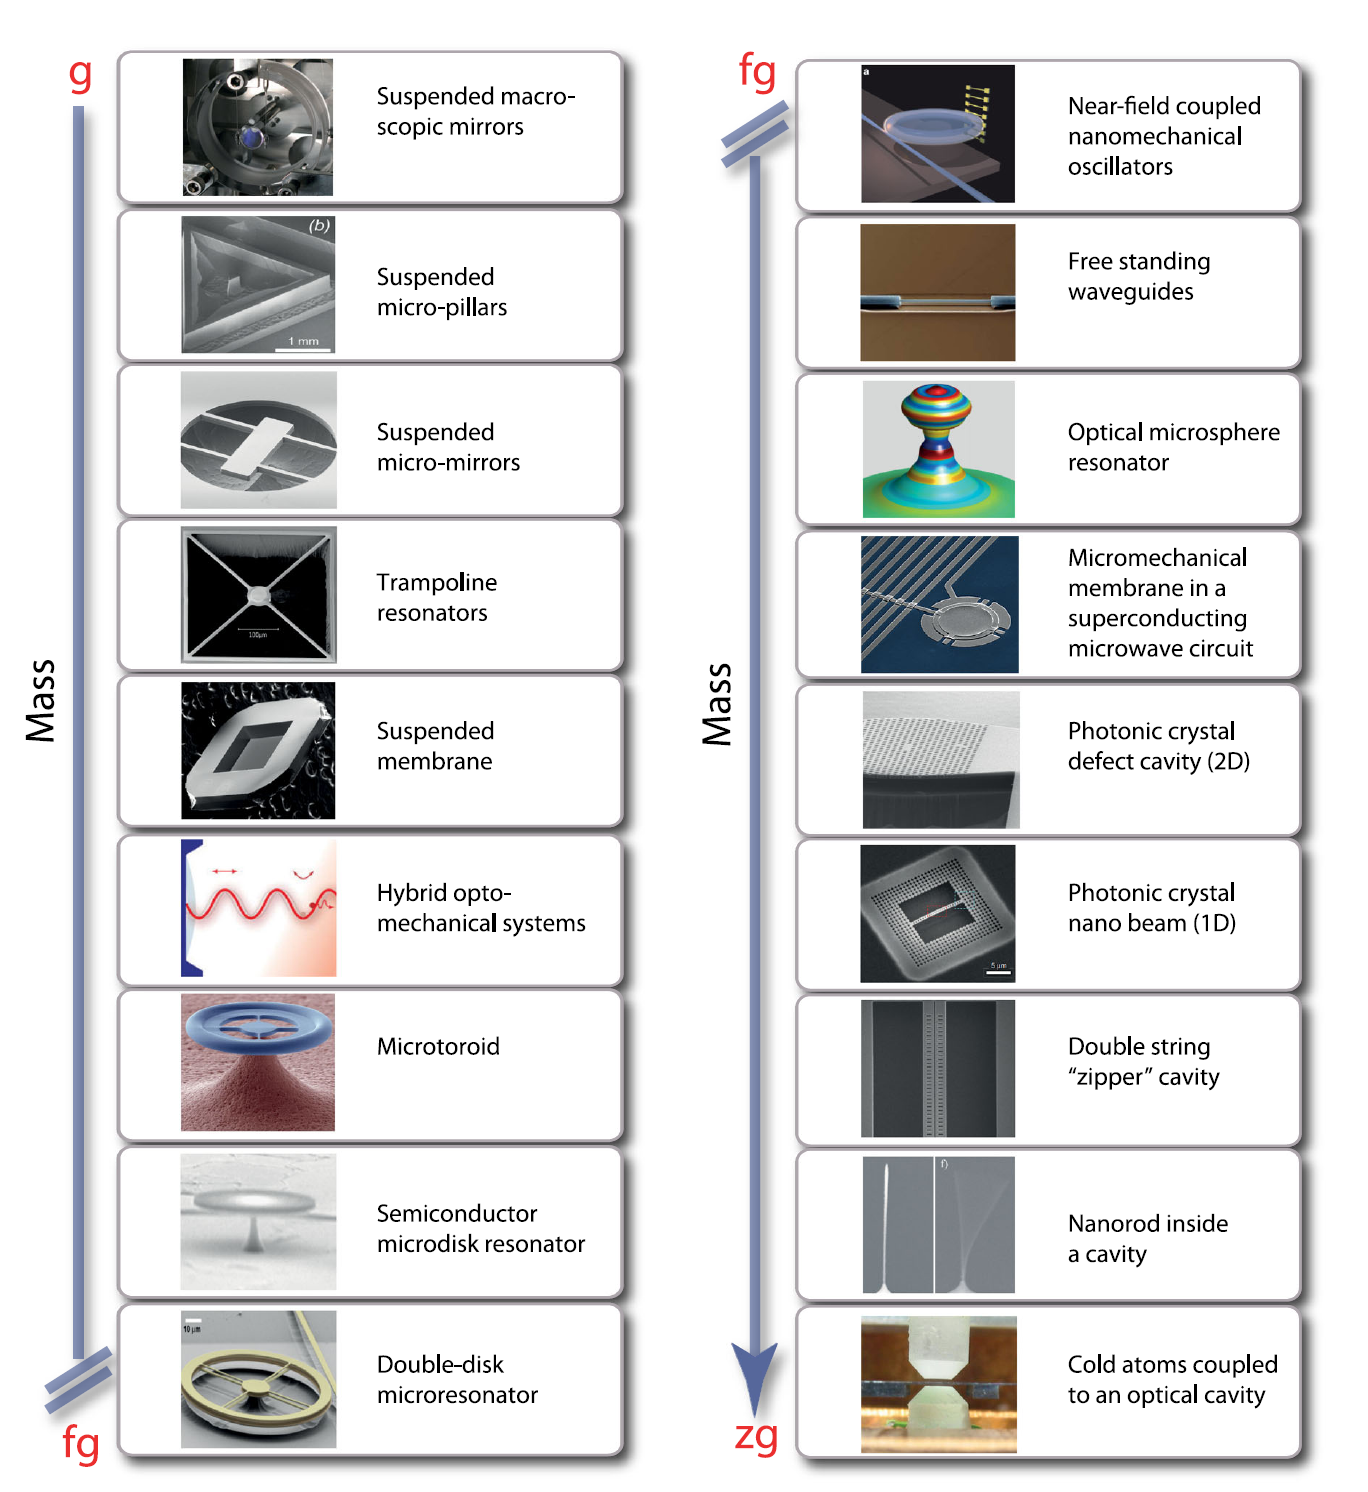
\includegraphics[width=3.5in]{optoMechDevices.png}
			\caption{A gallery illustrating the variety of optomechanical devices, arranged according to mass. \cite{Aspelmeyer2014} }
			\label{pic:optoMechDevices}
		\end{figure}

		\subsection{Parameters} % (fold)
		\label{sub:parameters}
			\begin{itemize}
				\item $ \Omega_m $: mechanical resonator frequency
				\item $ \Gamma_m = \Omega_m/Q_m $: mechanical dissipation rate
				\item $ \kappa $: optical dissipation rate
				\item $QF$ product: a direct measure for the degree of decoupling from the thermal environment
				\item $ g_0 $: bare optomechanical coupling rate
			\end{itemize}
		% subsection parameters (end)

		\subsection{Suspended mirrors} % (fold)
		\label{sub:suspended_mirrors}
			Suspend one of the cavity's mmirrors. The mechanical motion directly changes the cavity length and hence the frequency respond.

			purpose:
			\begin{itemize}
				\item laser interferometric detection of gravitational waves
				\item acoustic isolation
				\item quantum mechanical radiation-pressure fluctuations
				\item optical spring effect
				\item optical cooling
			\end{itemize}
		% subsection suspended_mirrors (end)

		\subsection{Optical microresonators} % (fold)
		\label{sub:optical_microresonators}
			Light is guided in whispering-gallery modes along the rim of a circular resonator. Distortions modify the optical path length of the resonator, shifting its optical frequency and generating optomechanical coupling.

			small size $ \rightarrow $ large $g_0$

			Three different architecture:
			\begin{enumerate}
				\item microdisk resonators: \\
				standard in planar photonic circuits\\
				$ g_0 \approx 2 \pi \times 8 \times 10^{5} $Hz\\
				fundamental limit: radiation losses at the sidewalls, internal material losses
				\item microsphere resonators:\\
				allow large optical quality\\
				mechanical quality mainly limited by internal material losses
				\item microtoroidal resonators:\\
				combination of high optical and mechanical quality\\
				first demonstrate r-p driven optomechanical parametric amplification
			\end{enumerate}

			Practical benefits of these geometries: large optical qualities with the resolved sideband regime $ \kappa<\Omega_m $

		% subsection optical_microresonators (end)


		\subsection{Waveguides and photonic crystal cavities} % (fold)
		\label{sub:waveguides_and}
		
		% subsection waveguides_and (end)


	% section experimental_realization (end)



	\bibliography{CavityOptomechanics}

\end{document}